
\chapter{Introduction}
\paragraph{What is this?}
These pages are a guide to tensors, using the visual language of ``tensor diagrams''.
For illustrating the generality of the approach, I've tried to closely follow the legendary ``Matrix Cookbook''.
As such, most of the presentation is a collection of facts (identities, approximations, inequalities, relations, ...) about tensors and matters relating to them.
You won't find many results not in the original cookbook, but hopefully the diagrams will give you a new way to understand and appreciate them.

\paragraph{It's ongoing:}
The Matrix Cookbook is a long book, and not all the sections are equally amenable to diagrams.
Hence I've opted to skip certain sections and shorten others.
Perhaps in the future, I, or others, will expand the coverage further.

For example, while we cover all of the results on Expectation of Linear Combinations and Gaussian moments, we skip the section on general multi-variate distributions.
I have also had to rearrange the material a bit, to avoid having to introduce all the notation up front.

\paragraph{Complex Matrices and Covariance}
Tensor diagrams (or networks) are currently most often seen in Quantum Physics,
but this is not a book for physicists.
The Matrix Cookbook is a book for engineers, in particular in Machine Learning, where complex numbers are less common.
Without complex numbers, we don't have to worry about complex conjugation, which simplifies transposes, and gets rid of the need for co- and contra-variant tensors.
% In particular transposing a matrix now involves taking the conjugate (flipping the sign of the imaginary part), which introduces the need for co- and contra-variant tensors.
% None of this complexity is present with standard real valued matrices, as is common e.g. in Machine Learning applications.
%For simplicity I have decided to not include these complexities.
If you are a physicist, you probably want a book on Tensor Analysis.

\paragraph{Tensorgrad}
The symbolic nature of tensor diagrams makes them well suited for symbolic computation.

\paragraph{Advantages of Tensor Diagram Notation:}
Tensor diagram notation has many benefits compared to other notations:

Various operations, such as a trace, tensor product, or tensor contraction can be expressed simply without extra notation.
Names of indices and tensors can often be omitted. This saves time and lightens the notation, and is especially useful for internal indices which exist mainly to be summed over.
The order of the tensor resulting from a complicated network of contractions can be determined by inspection: it is just the number of unpaired lines. For example, a tensor network with all lines joined, no matter how complicated, must result in a scalar.


\paragraph{Etymology}
The term "tensor" is rooted in the Latin word tensio, meaning ``tension'' or ``stretching,'' derived from the verb tendere, which means ``to stretch'' or ``to extend.''
It was first introduced in the context of mathematics in the mid-19th century by William Rowan Hamilton in his work on quaternions, where it referred to the magnitude of a quaternion.
The modern usage of "tensor" was later established by Gregorio Ricci-Curbastro and Tullio Levi-Civita in their development of tensor calculus, a framework that generalizes the concept of scalars, vectors, and matrices to more complex, multidimensional entities.~\cite{tensor_etymology_russo, hamilton_tensor}.


\tableofcontents
\clearpage


\section{Tensor Diagrams}
Tensor diagrams are simple graphs (or ``networks'') where
nodes represent variables (e.g. vectors or matrices) and edges represent
contractions (e.g. matrix multiplication or inner products.)
The following table shows how some basic operations can be written with tensor diagrams:

\newenvironment{compress}{
  \renewcommand{\arraystretch}{0.6} % Set the array stretch
  \setlength{\arraycolsep}{2pt}     % Set the column separation
  \vspace{.3em}
}{
  \vspace{.3em}
  \renewcommand{\arraystretch}{1}   % Reset to default after the environment
  \setlength{\arraycolsep}{5pt}     % Reset to default column separation
}

\renewcommand{\arraystretch}{2}
\noindent
%\hspace{-1em}
\vspace{.5em}
\begin{tabular}[h]{lcccl}
   Dot product
   &
   \begin{tikzpicture}[baseline=(a0.base), inner sep=1pt]
      \node (a0) {$a$};
      \node[right=1em of a0] (a1) {$b$};
      \path (a0) edge (a1);
   \end{tikzpicture}
   &
   $y=\sum_i a_i b_i$
   &
   $
\begin{compress}
\left[\begin{array}{cccc}
\cdot & \cdot & \cdot & \cdot \\
\end{array}\right]
\left[\begin{array}{c}
\cdot \\
\cdot \\
\cdot \\
\cdot \\
\end{array}\right]
\end{compress}
   $
   &
   $=y$
   \\
   Outer product
   &
   \begin{tikzpicture}[baseline=(a0.base), inner sep=1pt]
      \node (a0) {$a$};
      \node[right=.5em of a0] (a1) {$b$};
      \draw (a0.west) -- ++(-.3,0) node {};
      \draw (a1.east) -- ++(.3,0) node {};
   \end{tikzpicture}
   &
   $Y_{i,j} = a_i b_j$
   &
   $
\begin{compress}
\left[\begin{array}{c}
\cdot \\
\cdot \\
\cdot \\
\cdot \\
\end{array}\right]
\left[\begin{array}{cccc}
\cdot & \cdot & \cdot & \cdot \\
\end{array}\right]
\end{compress}
   $
   &
   $=\mathbin{
   \begin{tikzpicture}[baseline=(Y.base), inner sep=1pt]
      \node (Y) {$Y$};
      \draw (Y.east) -- ++(.3, 0);
      \draw (Y.west) -- ++(-.3, 0);
   \end{tikzpicture}}
   $
   \\
   Matrix-Vector
   &
   \begin{tikzpicture}[baseline=(A.base), inner sep=1pt]
      \node (A) {$A$};
      \node[right=.5em of A] (b) {$b$};
      \draw (A.west) -- ++(-.3,0) node {};
      \draw (A.east) -- (b.west);
   \end{tikzpicture}
   &
   $
   y_{i} = \sum_j A_{i,j} b_j
   $
   &
   $
   \begin{compress}
   \left[\begin{array}{cccc}
   \cdot & \cdot & \cdot & \cdot \\
   \cdot & \cdot & \cdot & \cdot \\
   \cdot & \cdot & \cdot & \cdot \\
   \cdot & \cdot & \cdot & \cdot \\
   \end{array}\right]
   \left[\begin{array}{c}
   \cdot \\
   \cdot \\
   \cdot \\
   \cdot \\
   \end{array}\right]
   \end{compress}
   $
   &
   $=\mathbin{
   \begin{tikzpicture}[baseline=(y.base), inner sep=1pt]
      \node (y) {$y$};
      \draw (y.west) -- ++(-.3, 0);
   \end{tikzpicture}
   }$
   \\
   Matrix-Matrix
   &
   \begin{tikzpicture}[baseline=(A.base), inner sep=1pt]
      \node (A) {$A$};
      \node[right=.5em of A] (B) {$B$};
      \draw (A.west) -- ++(-.3,0) node {};
      \draw (A.east) -- (B.west);
      \draw (B.east) -- ++(.3,0) node {};
   \end{tikzpicture}
   &
   $
   Y_{i,k} = \sum_j A_{i,j} B_{j,k}
   $
   &
   $
   \begin{compress}
   \left[\begin{array}{cccc}
   \cdot & \cdot & \cdot & \cdot \\
   \cdot & \cdot & \cdot & \cdot \\
   \cdot & \cdot & \cdot & \cdot \\
   \cdot & \cdot & \cdot & \cdot \\
   \end{array}\right]
   \left[\begin{array}{cccc}
   \cdot & \cdot & \cdot & \cdot \\
   \cdot & \cdot & \cdot & \cdot \\
   \cdot & \cdot & \cdot & \cdot \\
   \cdot & \cdot & \cdot & \cdot \\
   \end{array}\right]
   \end{compress}
   $
   &
   $=\mathbin{
   \begin{tikzpicture}[baseline=(Y.base), inner sep=1pt]
      \node (Y) {$Y$};
      \draw (Y.west) -- ++(-.3, 0);
      \draw (Y.east) -- ++(.3, 0);
   \end{tikzpicture}
   }$
\end{tabular}
\vspace{.5em}

We think of vectors and matrices as tensors of order 1 and 2.
The order corresponds to the number of dimensions in their $[\cdots]$ visualization above,
e.g. a vector is a 1-dimensional list of numbers, while a matrix is a 2-dimensional grid of numbers.
The order also determines the degree of the node representing the variable in the tensor graph.

Diagram notation becomes more interesting when you have tensors of order 3 and higher.
An order 3 tensor is a cube or numbers, or stack of matrices.
E.g. we can write this as $T\in\R^{n\times m\times k}$, so $T_i\in\R^{m\times k}$ is a matrix for $i=1\dots n$.
Of course we could slice $T$ along the other axes too, so $T_{:,j}\in\R^{n\times k}$ and $T_{:,:,\ell}\in\R^{n\times m}$ are matrices too.

A matrix having two outgoing edges means there are two ways you can multiply a vector onto it, either on the left: $x^T M$, or on the right: $Mx$.
In graph notation we just write $x\!-\!M\!-$ and $-M\!-\!x$.
An order 3 tensor has three edges, so we can multiply it with a vector in three ways:
\[
   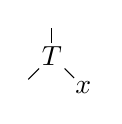
\begin{tikzpicture}[baseline=(T.base), inner sep=1pt]
      \node (T) {$T$};
      \node (x) at (.4,-.4) {$x$};
      \draw (T) -- (x);
      \draw (T) -- ++(-.3,-.3);
      \draw (T) -- ++(0,.35);
   \end{tikzpicture}
   \quad
   \text{and}
   \quad
   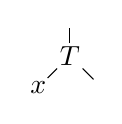
\begin{tikzpicture}[baseline=(T.base), inner sep=1pt]
      \node (T) {$T$};
      \node (x) at (-.4,-.4) {$x$};
      \draw (T) -- (x);
      \draw (T) -- ++(.3,-.3);
      \draw (T) -- ++(0,.35);
   \end{tikzpicture}
   \quad
   \text{and}
   \quad
   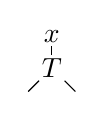
\begin{tikzpicture}[baseline=(T.base), inner sep=1pt]
      \node (T) {$T$};
      \node (x) at (0,.4) {$x$};
      \draw (T) -- (x);
      \draw (T) -- ++(.3,-.3);
      \draw (T) -- ++(-.3,-.3);
   \end{tikzpicture}
\]
%
To be perfectly precise about what each one means, we should give the edges labels.
For example we would write
$
   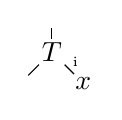
\begin{tikzpicture}[baseline=(T.base), inner sep=1pt]
      \node (T) {$T$};
      \node (x) at (.4,-.4) {$x$};
      \draw (T) -- (x) node[midway, above right, font=\tiny] {i};
      \draw (T) -- ++(-.3,-.3);
      \draw (T) -- ++(0,.3);
   \end{tikzpicture}
$
to specify the matrix $\sum_i T_i x_i$.
However, often the edge in question will be clear from the context, which is part of
what makes tensor diagram notation cleaner than, say, Einstein sum notation.

\[
   Y_{i,j} = \sum_{k,l,m,n,o} A_{i,k} B_{l,n,o} C_{j,k,l,m} D_{m,n} E_o
   \quad
   \Leftrightarrow
   % \quad
   \vcenter{\hbox{
      \import{figures/}{basic_graph.pdf_tex}
   }}
\]

The \emph{key principle} of tensor diagrams is that \emph{edge contraction is associative}.
This means you can contract any edge in any order you prefer.
This can be seen from the sum representation above, which can be reordered to sum over $k,l,m,n$ in any order.

The computational price for different contraction orders can be widely different.
Unfortunately it's not computationally easy to find the optimal order.
See section~\ref{sec:opt_contr} for algorithms to find the best contraction order, and approximate contraction methods.

Note that tensor graphs are not always connected.
We already saw that the outer product of two vectors can be written
   $\begin{tikzpicture}[baseline=(a0.base), inner sep=1pt]
      \node (a0) {$a$};
      \node[right=.5em of a0] (a1) {$b$};
      \draw (a0.west) -- ++(-.3,0) node {};
      \draw (a1.east) -- ++(.3,0) node {};
   \end{tikzpicture}$.
This is natural from the sum representation: No edges simply means no sums.
So here $y_{i,j} = a_i b_j$, which is exactly the outer product $y=a\otimes b$.
% Can also mention how this gives us scaling by letter (5) be the order-0 tensor with value 5.


\section{The Copy Tensor}

A particularly important tensor is the ``copy'' tensor, also known as the ``diagonal'', ``kronecker delta'' or ``spider'' tensor.
The simplest version is the all-ones vector, which we write as $\sbullet-$.
That is $\sbullet_i = 1$.
The general order-n tensor is 1 on the diagonal, 0 everywhere else:
\[
   \sbullet_{i,j,k,\ldots} = \begin{cases}
      1\quad \text{if } i=j=k=\dots \\
      0\quad \text {otherwise}
   \end{cases}
\]
% This is also known as the ``copy'' or ``spider'' tensor, or ``generalized Kronecker delta''.
Or, using Iversonian notation,\footnote{%
For a logical proposition $P$, we define $
   [P] = \begin{cases}
      1 \text{ if } P \\
      0 \text{ otherwise}
   \end{cases}
$.} $\sbullet_{i,j,k,\dots} = [i=j=k=\dots]$.
We see the order-2 copy-tensor, $-\sbullet- = I$, is just the identity matrix,
so we can simply remove it from graphs like this:
\[-A\!-\!\sbullet\!-\!B- = -A\!-\!B-\]

Higher order copy-tensors are very useful, because they let us turn the simple tensor graphs into hyper-graphs.
A simple example of how we can use this is the diagonal matrix $D_a$, which has $a$ on the diagonal and 0 elsewhere.
We can write this as
\[
   D_a = 
   \begin{tikzpicture}[baseline=(T.base), inner sep=1pt]
      \node (T) {$\sbullet$};
      \node (x) at (.3,-.3) {$a$};
      \draw (T) -- (x);
      \draw (T) -- ++(-.25,-.25);
      \draw (T) -- ++(0,.3);
   \end{tikzpicture}
\]
Why?
Because $(D_a)_{i,j} = \sum_k \sbullet_{i,j,k} a_k = \sum_k [i=j=k] a_k = [i=j] a_i$.
Similarly the Hadamard product, $(a\circ b)_i = a_i b_i$, can be written
\[
   a \circ b =
   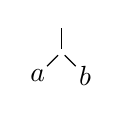
\begin{tikzpicture}[baseline=(T.base), inner sep=1pt]
      \node (T) {$\sbullet$};
      \node (a) at (-.3,-.3) {$a$};
      \node (b) at (.3,-.3) {$b$};
      \draw (T) -- (a);
      \draw (T) -- (b);
      \draw (T) -- ++(0,.3);
   \end{tikzpicture}
\]
Now, let's see why everyone loves copy tensors by using it to
prove the identity $D_aD_b = D_{a\circ b}$ by ``copy tensor manipulation'':
\[
   D_a D_b =
   \begin{tikzpicture}[baseline=(T.base), inner sep=1pt]
      \node (T) {$\sbullet$};
      \node (a) at (-.3,-.3) {$a$};
      \draw (T) -- (a);
      \node (T2) at (.5,0) {$\sbullet$};
      \node (b) at (.8,-.3) {$b$};
      \draw (T) -- ++(0,.3);
      \draw (T) -- (T2);
      \draw (T2) -- (b);
      \draw (T2) -- ++(0,.3);
   \end{tikzpicture}
   =
   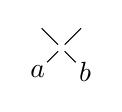
\begin{tikzpicture}[baseline=(T.base), inner sep=1pt]
      \node (T) {$\sbullet$};
      \node (a) at (-.3,-.3) {$a$};
      \node (b) at (.3,-.3) {$b$};
      \draw (T) -- (a);
      \draw (T) -- (b);
      \draw (T) -- ++(.25,.25);
      \draw (T) -- ++(-.25,.25);
   \end{tikzpicture}
   =
   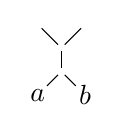
\begin{tikzpicture}[baseline=(T.base), inner sep=1pt]
      \node (T) {$\sbullet$};
      \node (a) at (-.3,-.3) {$a$};
      \node (b) at (.3,-.3) {$b$};
      \draw (T) -- (a);
      \draw (T) -- (b);
      \node (T2) at (0,.3) {$\sbullet$};
      \draw (T) -- (T2);
      \draw (T2) -- ++(.25,.25);
      \draw (T2) -- ++(-.25,.25);
   \end{tikzpicture}
   =
   D_{a\circ b}.
\]
You can verify this using the sum representation.

The general rule at play is that any connected sub-graph of copy-tensors can be combined into a single one.
Sometimes we are even lucky enough that this simplification leaves us with an identity matrix we can remove too:
%\begin{figure}[h]
%   \centering{
   %\def\svgwidth{.5\linewidth}
   %\import{figures/}{path1.pdf_tex}
   %\\
\[
   \def\svgwidth{.75\linewidth}
   \import{figures/}{path2.pdf_tex}
   .
\]
%   \caption{Contracting copy tensors and identity matrices}
%   \label{fig:spiders}
%   }
%\end{figure}
The only time you have to be a bit careful is when the resulting tensor has order 0.
Depending on how you define the order-0 copy tensor, $\sbullet$, you may or may not have the identity $\sbullet\!-\!\sbullet = \sbullet$.

Lots of other constructions that require special notation (like diagonal matrices or Hadamard products) with normal vector notation can be unified using the copy tensor.
%
In the Matrix Cookbook they define the order-4 tensor $J$,
which satisfies $J_{i,j,k,l} = [i=k][j=l]$ and which we'd write as
$J=\vcenter{\hbox{
   \begin{tikzpicture}[inner sep=0pt]
   \node (a0) {$\sbullet$};
   \draw (a0.east) -- ++(.2,0);
   \draw (a0.west) -- ++(-.2,0);
   \node[below=.2em of a0] (a1) {$\sbullet$};
   \draw (a1.east) -- ++(.2,0);
   \draw (a1.west) -- ++(-.2,0);
\end{tikzpicture}}}$,
and satisfies, for example, $\frac{dX}{dX}=J$.
Using ``tensor products'' you could write $J=I\otimes I$.
Note that $J$ is different from the order-4 copy-tensor,

\begin{tikzpicture}[baseline=(a0.base), inner sep=0pt]
   \node (a0) {$\sbullet$};
   \draw (a0) -- ++(.17,.17);
   \draw (a0) -- ++(.17,-.17);
   \draw (a0) -- ++(-.17,.17);
   \draw (a0) -- ++(-.17,-.17);
\end{tikzpicture}.

\section{Sums of Tensors}

Tensor products can express any linear function.
That is $f$ such that $f(a x, b y) = a b f(x,y)$.
Unfortunately not all operations on tensors are linear.
Even something as simple as a sum of two vectors, $x+y$, can not be displayed with a simple contraction graph.
(Note that this is not linear because $ax+by\neq ab(x+y)$.)

To handle this important operation, Penrose suggesting simply writing the two graphs with a plus sign between them, such as $-x + -y$.
Note that this is itself an order-1 tensor, even though it may look like there are two free edges.
If we want to multiply the sum with another tensor, we can use parentheses like $-M\!-\!(-x + -y)$.

It can be helpful to use named edges when dealing with sums, to make it clear how the edges are matched up.
Sums and tensor products interact nicely, with a general form of the distributive law:
%\begin{figure}[h]
%\centering{
%\def\svgwidth{\linewidth}
\[
\def\svgwidth{.75\linewidth}
\import{figures/}{path3.pdf_tex}
.
\]
%\caption{Distributive law}
%\label{fig:dist}
%}
%\end{figure}

When adding tensors that don't have the same number of edges, or have edges with different names, we can use ``broadcasting''.
%Say we want to add a matrix $\,_i\!-M-_j$ and a vector $x$.
Say we want to add a matrix $M$ and a vector $x$.
What does it even mean?
If we want to add $x$ to every row of $M$, we write
$
\vcenter{\hbox{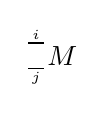
\begin{tikzpicture}[inner sep=1pt]
   \node (M) {$M$};
   \draw (M.north west) -- ++(-.2,0) node[midway, above, font=\tiny] {$i$};
   \draw (M.south west) -- ++(-.2,0) node[midway, below, font=\tiny] {$j$};
\end{tikzpicture}}}
+
\vcenter{\hbox{\begin{tikzpicture}[inner sep=1pt]
   \node (a0) {$\sbullet$};
   \draw (a0.west) -- ++(-.2,0) node[midway, above, font=\tiny] {$i$};
   \node[below=.2em of a0] (a1) {$x$};
   \draw (a1.west) -- ++(-.2,0) node[midway, below, font=\tiny] {$j$};
\end{tikzpicture}}}
$.
This is because
$
\vcenter{\hbox{\begin{tikzpicture}[inner sep=1pt]
   \node (a0) {$\sbullet$};
   \draw (a0.west) -- ++(-.2,0) node[midway, above, font=\tiny] {$i$};
   \node[below=.2em of a0] (a1) {$x$};
   \draw (a1.west) -- ++(-.2,0) node[midway, below, font=\tiny] {$j$};
\end{tikzpicture}}}
$
is an outer product between $x$ and the all one vector, which is a matrix in which every row is the same.
Similarly, if we want to add $x$ to every column, we could use
the matrix
$
\vcenter{\hbox{\begin{tikzpicture}[inner sep=1pt]
   \node (a0) {$\sbullet$};
   \draw (a0.west) -- ++(-.2,0) node[midway, below, font=\tiny] {$j$};
   \node[above=.2em of a0] (a1) {$x$};
   \draw (a1.west) -- ++(-.2,0) node[midway, above, font=\tiny] {$i$};
\end{tikzpicture}}}
$.

Note that we typically don't talk about ``rows'' or ``columns'' when dealing with tensors, but simply use the name edge (sometimes axis) of the tensor.
When using named edges, operations from classical vector notation like ``transpose'' can also be removed.
The matrix $X^T$ is simply $X$ where the left and right edge have been swapped.
But if the edges are named, we don't have to keep track on ``where the edge is'' at all.

\section{Transposition}
In classical matrix notation, transposition flips the indices of a matrix, so that
\[
   (A^T)_{ij} = A_{ji}.
\]
In tensor diagram notation, we have two choices depending on whether we want the position of the edges to be significant.
With significant edge positions, we typically let the ``left edge'' be the first index, and the ``right edge'' be the second index.
Thus transposition requires flipping the edges:
\[
   (\matmul{A})^T
   =
   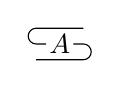
\begin{tikzpicture}[baseline=(a0.base), inner sep=1pt]
      \node (a0) {$A$};
      \draw (a0) -- ++(.3, 0) arc (270:90:-.1) --  ++(-.6, 0);
      \draw (a0) -- ++(-.3, 0) arc (270:90:.1) --  ++(.6, 0);
   \end{tikzpicture}
   =
   \matmul{A^T}.
\]
A fun notation used by some authors is flipping the tensor upside down, $\matmul{\vflip{A}}$, as a simpler way to flip the left and right edges.

In practical computations, keeping track of the edge positions can be easy to mess up.
It's more robust to name the ``outputs'' of the tensor, and let transposition rename the edges:
\[
   (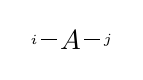
\begin{tikzpicture}[baseline=(A.base), inner sep=1pt]
   \node (A) {$A$};
   \draw (A.west) -- ++(-.2,0) node[left, font=\tiny] {$i$};
   \draw (A.east) -- ++(.2,0) node[right, font=\tiny] {$j$};
\end{tikzpicture})^T
=
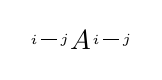
\begin{tikzpicture}[baseline=(A.base), inner sep=1pt]
   \node (A) {$A$};
   \node[font=\tiny] (i) at (-.2,0) {$j$};
   \node[font=\tiny] (j) at (.2,0) {$i$};
   \draw (i.west) -- ++(-.2,0) node[left, font=\tiny] {$i$};
   \draw (j.east) -- ++(.2,0) node[right, font=\tiny] {$j$};
\end{tikzpicture}
\]
%
Renaming can be done using multiplication by identity matrices:
\[
(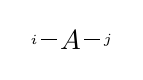
\begin{tikzpicture}[baseline=(A.base), inner sep=1pt]
   \node (A) {$A$};
   \draw (A.west) -- ++(-.2,0) node[left, font=\tiny] {$i$};
   \draw (A.east) -- ++(.2,0) node[right, font=\tiny] {$j$};
\end{tikzpicture})
(
\begin{tikzpicture}[baseline=(A.base), inner sep=1pt]
   \node (A) {$\sbullet$};
   \draw (A.west) -- ++(-.2,0) node[left, font=\tiny] {$j$};
   \draw (A.east) -- ++(.2,0) node[right, font=\tiny] {$k$};
\end{tikzpicture})
=
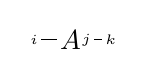
\begin{tikzpicture}[baseline=(A.base), inner sep=1pt]
   \node (A) {$A$};
   \draw (A.west) -- ++(-.2,0) node[left, font=\tiny] {$i$};
   \node[font=\tiny] (j) at (.2,0) {$j$};
   \draw (j) -- ++(.2,0) node[right, font=\tiny] {$k$};
\end{tikzpicture},
\]
but we have to be careful because overlapping edge names can make multiplication non-associative.
E.g.
\[
   \big[
(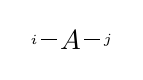
\begin{tikzpicture}[baseline=(A.base), inner sep=1pt]
   \node (A) {$A$};
   \draw (A.west) -- ++(-.2,0) node[left, font=\tiny] {$i$};
   \draw (A.east) -- ++(.2,0) node[right, font=\tiny] {$j$};
\end{tikzpicture})
(
\begin{tikzpicture}[baseline=(A.base), inner sep=1pt]
   \node (A) {$\sbullet$};
   \draw (A.west) -- ++(-.2,0) node[left, font=\tiny] {$j$};
   \draw (A.east) -- ++(.2,0) node[right, font=\tiny] {$k$};
\end{tikzpicture})
\big]
(
\begin{tikzpicture}[baseline=(A.base), inner sep=1pt]
   \node (A) {$\sbullet$};
   \draw (A.west) -- ++(-.2,0) node[left, font=\tiny] {$k$};
   \draw (A.east) -- ++(.2,0) node[right, font=\tiny] {$j$};
\end{tikzpicture})
=
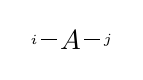
\begin{tikzpicture}[baseline=(A.base), inner sep=1pt]
   \node (A) {$A$};
   \draw (A.west) -- ++(-.2,0) node[left, font=\tiny] {$i$};
   \draw (A.east) -- ++(.2,0) node[right, font=\tiny] {$j$};
\end{tikzpicture}
\neq
(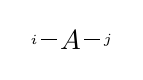
\begin{tikzpicture}[baseline=(A.base), inner sep=1pt]
   \node (A) {$A$};
   \draw (A.west) -- ++(-.2,0) node[left, font=\tiny] {$i$};
   \draw (A.east) -- ++(.2,0) node[right, font=\tiny] {$j$};
\end{tikzpicture})
   \big[
(
\begin{tikzpicture}[baseline=(A.base), inner sep=1pt]
   \node (A) {$\sbullet$};
   \draw (A.west) -- ++(-.2,0) node[left, font=\tiny] {$j$};
   \draw (A.east) -- ++(.2,0) node[right, font=\tiny] {$k$};
\end{tikzpicture})
(
\begin{tikzpicture}[baseline=(A.base), inner sep=1pt]
   \node (A) {$\sbullet$};
   \draw (A.west) -- ++(-.2,0) node[left, font=\tiny] {$k$};
   \draw (A.east) -- ++(.2,0) node[right, font=\tiny] {$j$};
\end{tikzpicture})
\big]
=
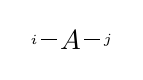
\begin{tikzpicture}[baseline=(A.base), inner sep=1pt]
   \node (A) {$A$};
   \draw (A.west) -- ++(-.2,0) node[left, font=\tiny] {$i$};
   \draw (A.east) -- ++(.2,0) node[right, font=\tiny] {$j$};
\end{tikzpicture}
\,
\begin{tikzpicture}[baseline=-0.6em, inner sep=1pt]
   \node (a0) {$\sbullet$};
   \node[below=.1 of a0] (a1) {$\sbullet$};
   \draw (a0) -- ++(.1, 0) arc (270:90:-.15) -- (a1);
   \draw (a1) -- ++(-.1, 0) arc (270:90:.15) -- (a0);
\end{tikzpicture},
\]
where
$\begin{tikzpicture}[baseline=-0.7em, inner sep=1pt]
   \node (a0) {$\sbullet$};
   \node[below=.1 of a0] (a1) {$\sbullet$};
   \draw (a0) -- ++(.1, 0) arc (270:90:-.15) -- (a1);
   \draw (a1) -- ++(-.1, 0) arc (270:90:.15) -- (a0);
\end{tikzpicture}$
equals the matrix dimension.
In tensorgrad we solve this problem by requiring that any edge name is present at most twice in any product.

For the purpose of transcribing the matrix cookbook, using the ``significant position'' notation is more convenient.
We observe the following identities:
\begin{walign}
(A^T)^T &= A 
&
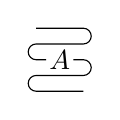
\begin{tikzpicture}[baseline=(a0.base), inner sep=1pt]
   \node (a0) {$A$};
   \draw (a0) -- ++(.3, 0) arc (270:90:-.1) -- ++(-.6, 0) arc (90:270:.1) -- ++(.6, 0);
   \draw (a0) -- ++(-.3, 0) arc (270:90:.1) -- ++(.6, 0) arc (90:270:-.1) -- ++(-.6, 0);
\end{tikzpicture}
&=
\matmul{A}
\\
%%%%%%%%%%%%%%%%%%%%%%%%%%%%%%%%%%%%%%%%%%%%%%%%%%%%%%%%%%%%%%%%%%%%%%%%%%%%%%%%
\tag{4}
(A + B)^T &= A^T + B^T
&
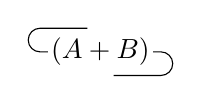
\begin{tikzpicture}[baseline=(a0.base), inner sep=1pt]
   \node (a0) {$\left( \matmul{A} + \matmul{B} \right)$};
   \draw (a0.east) -- ++(.1, 0) arc (270:90:-.15) -- ++(-.6, 0);
   \draw (a0.west) -- ++(-.1, 0) arc (270:90:.15) -- ++(.6, 0);
\end{tikzpicture}
&=
   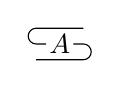
\begin{tikzpicture}[baseline=(a0.base), inner sep=1pt]
      \node (a0) {$A$};
      \draw (a0) -- ++(.3, 0) arc (270:90:-.1) --  ++(-.6, 0);
      \draw (a0) -- ++(-.3, 0) arc (270:90:.1) --  ++(.6, 0);
   \end{tikzpicture}
+
   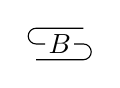
\begin{tikzpicture}[baseline=(a0.base), inner sep=1pt]
      \node (a0) {$B$};
      \draw (a0) -- ++(.3, 0) arc (270:90:-.1) --  ++(-.6, 0);
      \draw (a0) -- ++(-.3, 0) arc (270:90:.1) --  ++(.6, 0);
   \end{tikzpicture}
%\\
\end{walign}
\begin{walign}
%%%%%%%%%%%%%%%%%%%%%%%%%%%%%%%%%%%%%%%%%%%%%%%%%%%%%%%%%%%%%%%%%%%%%%%%%%%%%%%%
\tag{5}
(AB)^T &= B^T A^T
&
   \begin{tikzpicture}[baseline=(a.base), inner sep=1pt]
      \node (a) {$A$};
      \node[right=.5em of a] (b) {$B$};
      \draw (a) -- (b);
      \draw (b) -- ++(.3, 0) arc (270:90:-.1) --  ++(-.6, 0);
      \draw (a) -- ++(-.3, 0) arc (270:90:.1) --  ++(.6, 0);
   \end{tikzpicture}
&=
\begin{tikzpicture}[baseline=-.8em, inner sep=1pt]
   \node (a) {\vflip{$A$}};
   \node[below=.3em of a] (b) {\vflip{$B$}};
   \draw (a) -- ++(.3, 0);
   \draw (a) -- ++(-.3, 0) arc (90:270:.1) -- ++(.6, 0) arc (270:90:-.1) -- (b);
   \draw (b) -- ++(-.3, 0);
\end{tikzpicture}
=
\matmul{ \vflip{B}, \vflip{A} }
\end{walign}

\subsection{Higher order}
It is possible to generalize the idea of a transpose to higher order tensors.
It requires partitioning the edges as ``input'' and ``output'' edges, or more commonly, ``contravariant'' and ``covariant'' edges.
See the section at the end of this chapter for more on this.

We say matrices are symmetric if $A^T = A$.
For higher order tensors, there are many ways to be symmetric.
See the section~\ref{sec:symmetry} for more on this.

\section{Trace}

The ``trace'' of a square matrix is defined $\mathrm{Tr}(A) = \sum_i A_{i,i}$.
In tensor diagram notation, that corresponds to a self-edge: $\trace{A}{1}$.
The Matrix Cookbook has a list of identities using traces.
Let's reproduce them with tensor diagrams:
\begin{walign}
   \tag{11}
   \sum_{i=1}^{n} A_{ii} &= \mathrm{Tr}(A) = \mathrm{Tr}(A I)
   &
   \trace{A}{1} &= \trace{A, \sbullet}{2}
   \\
   %%%%%%%%%%%%%%%%%%%%%%%%%%%%%%%%%%%%%%%%
   \tag{13}
   \mathrm{Tr}(A) &= \mathrm{Tr}(A^T)
   &
   \trace{A}1
   \hspace{-1em}
   &=
   \hspace{-1em}
   \vflip{\trace{A}1}
   \\[0.5em]
   %%%%%%%%%%%%%%%%%%%%%%%%%%%%%%%%%%%%%%%%
   \tag{14}
   \mathrm{Tr}(AB)
   &=
   \mathrm{Tr}(BA)
   &
   \trace{A,B}2
   \hspace{-.5em}
   &=
   \hspace{.5em}
   \begin{tikzpicture}[baseline=-1em, inner sep=1pt]
      \node (a) {$\vflip{B}$};
      \node[below=.3em of a] (b) {$A$};
      \draw (a) -- ++(-.3, 0) arc (90:270:.2) -- (b);
      \draw (a) -- ++(.3, 0) arc (270:90:-.2) -- (b);
   \end{tikzpicture}
   \hspace{.5em}
   =
   \hspace{-.5em}
   \trace{B,A}2
   \\[0.5em]
   %%%%%%%%%%%%%%%%%%%%%%%%%%%%%%%%%%%%%%%%
   \tag{15}
   \mathrm{Tr}(A+B)
   &= \mathrm{Tr}(A) + \mathrm{Tr}(B)
   &
   %\trace{(A+B),\sbullet}1
   %\trace{(\matmul{A}+\matmul{B}),\sbullet}1
   %\trace{(\matmul{A}+\matmul{B})}1
   %\trace{(\matmul{A}+\matmul{B}),\sbullet}{2}
   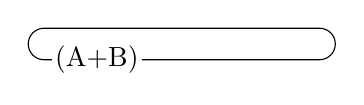
\begin{tikzpicture}[baseline=(a.base), inner sep=1pt]
      \node (a) {(\matmul{A}+\matmul{B})};
      \draw (a.west) -- ++(-.1, 0) arc (270:90:.2) -- ++(3.5, 0) arc (270:90:-.2) -- (a.east);
   \end{tikzpicture}
   &=
   \hspace{-1em}
   \trace{A}1
   \hspace{-1em}
   +
   \hspace{-1em}
   \trace{B}1
   \hspace{-1em}
   \\[0.5em]
   %%%%%%%%%%%%%%%%%%%%%%%%%%%%%%%%%%%%%%%%
   \tag{16}
   \mathrm{Tr}(ABC) &= \mathrm{Tr}(BCA)
   &
   \trace{A,B,C}1 &= \trace{B,C,A}1
   \\
                  & = \mathrm{Tr}(CAB)
                  &&= \trace{C,A,B}1
   \\[0.5em]
   %%%%%%%%%%%%%%%%%%%%%%%%%%%%%%%%%%%%%%%%
   \tag{17}
   a^T a &= \mathrm{Tr}(a a^T)
   &
   \vecmatvec{1em}{a}{}{a}
   &=
   \mathrm{Tr}(
   \begin{tikzpicture}[baseline=(a0.base), inner sep=1pt]
      \node (a0) {$a$};
      \node[right=.5em of a0] (a1) {$a$};
      \draw (a0.west) -- ++(-.3,0) node {};
      \draw (a1.east) -- ++(.3,0) node {};
   \end{tikzpicture}
   )
 \\&&&=
   \hspace{-1em}
   \begin{tikzpicture}[baseline=(a0.base), inner sep=1pt]
      \node (a0) {$a$};
      \node[right=1em of a0] (a1) {$a$};
      \path (a0) edge [out=160, in=20, looseness=2] (a1);
   \end{tikzpicture}
   \hspace{-1em}
\end{walign}

\subsection{Higher order traces}
For higher order tensors, we still define the trace as the sum of the diagonal elements.
That is, for a tensor $A$ of order $n$, the trace is just the product with the order $n$ copy tensor:
\[
   \begin{tikzpicture}[baseline=(T.base), inner sep=1pt]
      \node (Tr) {Tr(};
      \node[right=.3em of Tr] (T) {$T$};
      \node[right=.3em of T] (p) {)};
      \draw (T) -- ++(.3,-.3);
      \draw (T) -- ++(-.3,-.3);
      \draw (T) -- ++(0,.35);
   \end{tikzpicture}
   =
   \begin{tikzpicture}[baseline=(T.base), inner sep=1pt]
      \node (T) {$T$};
      \node[right=2em of T] (s) {$\sbullet$};
      \path (T) edge [out=90, in=120] (s);
      \path (T) edge [out=-30, in=200] (s);
      \path (T) edge [out=-120, in=220] (s);
   \end{tikzpicture}
   .
\]
In quantum mechanics, it is common to use a ``partial trace'', which we can define using index notation:
\[
   \begin{tikzpicture}[baseline=(T.base), inner sep=1pt]
      \node (Tr) {Tr$_{i,j}$(};
      \node[right=.3em of Tr] (T) {$T$};
      \node[right=.3em of T] (p) {)};
      \draw (T) -- ++(.3,-.3) node[midway, below left, font=\tiny] {j};
      \draw (T) -- ++(-.3,-.3) node[midway, below right, font=\tiny] {i};
      \draw (T) -- ++(0,.35) node[midway, above right, font=\tiny] {k};
   \end{tikzpicture}
   =
   \hspace{-.5em}
   \begin{tikzpicture}[baseline=(T.base), inner sep=1pt]
      \node (T) {$T$};
      \draw (T) -- ++(0,.35) node[midway, above right, font=\tiny] {k};
      \path (T) edge [out=-120, in=-60, loop] (T);
   \end{tikzpicture}
   .
\]
Of course with tensor diagrams, we can also use partial traces without naming the indices.
We don't even have to think about whether the contractions we use are traces or not.

\section{Eigenvalues}
Eigenvalues and eigenvectors are fundamental concepts in linear algebra that have important applications in tensor network theory. In tensor diagram notation, we can represent these concepts in a visually intuitive way.

For a matrix $A$, if there exists a non-zero vector $v$ and a scalar $\lambda$ such that $Av = \lambda v$, then $\lambda$ is called an eigenvalue of $A$, and $v$ is the corresponding eigenvector.
In tensor diagram notation It's convenient to write its eigendecomposition as $A = Q\Lambda Q^{-1}$, where $Q$ is a matrix whose columns are the eigenvectors of $A$, and $\Lambda$ is a diagonal matrix of the eigenvalues.
Thus:
\begin{align}
   \label{eq:eigen-decomposition}
   \begin{tikzpicture}[baseline=(A.base), inner sep=1pt]
   \node (A) {$A$};
   \draw (A.west) -- ++(-.3, 0);
   \draw (A.east) -- ++(+.3, 0);
   \end{tikzpicture}
   =
   \begin{tikzpicture}[baseline=(Q.base), inner sep=1pt]
   \node (Q) {$Q$};
   \draw (Q.west) -- ++(-.3, 0);
   \node[right=1em of Q] (dot) {$\sbullet$};
   \path (Q) edge (dot);
   \node[below=.3em of dot] (e) {$\lambda$};
   \path (dot) edge (e);
   \node[right=1em of dot] (Qi) {$Q^{-1}$};
   \path (dot) edge (Qi);
   \draw (Qi.east) -- ++(.3, 0);
   \end{tikzpicture}
\end{align}
The trace of a matrix is equal to the sum of its eigenvalues. We can represent this relationship using tensor diagrams:
\[
   \tag{12}
   \text{Tr}(A)
   =
   \hspace{-1em}
   \trace{A}{1}
   \hspace{-1em}
   =
   \hspace{-3em}
   \begin{tikzpicture}[baseline=(Q.base), inner sep=1pt]
      \node (Q) {$Q$};
      \node[right=1em of Q] (dot) {$\sbullet$};
      \path (Q) edge (dot);
      \node[below=.3em of dot] (e) {$\lambda$};
      \path (dot) edge (e);
      \node[right=1em of dot] (Qi) {$Q^{-1}$};
      \path (dot) edge (Qi);
      \path (Q.west) edge [out=160, in=20, looseness=2] (Qi.east);
   \end{tikzpicture}
   \hspace{-3em}
   =
   \hspace{-1em}
   \begin{tikzpicture}[baseline=(dot.base), inner sep=1pt]
      \node (dot) {$\sbullet$};
      \node[below=.3em of dot] (e) {$\lambda$};
      \path (dot) edge (e);
      \path (dot) edge [out=160, in=20, loop] ();
   \end{tikzpicture}
   \hspace{-1em}
   =
   \begin{tikzpicture}[baseline=(dot.base), inner sep=1pt]
      \node (dot) {$\sbullet$};
      \node[below=.3em of dot] (e) {$\lambda$};
      \path (dot) edge (e);
   \end{tikzpicture}
   =
   \sum_i \lambda_i
\]



\section{Symmetry and Symmetrization}
\label{sec:symmetry}

A common property of tensors is symmetry.
For matrices, symmetry means that $A^T = A$.
For tensors it means that permuting its indices does not change its value.
Typical examples are Covariance or Hessian matrices,
but also certain higher-order statistical moments, like the third or fourth moment tensors, can exhibit symmetries.
Sometimes only with respect to particular group, but most of the time with respect to all permutations of edges.
The Copy Tensor is a simple example of a completely symmetric tensor.

Sometimes it will be useful to symmetrize a tensor by summing over all permutations of its indices.
We write this using a squiggly line over the symmetrized edges:
\[
   \begin{tikzpicture}[baseline=.1em, inner sep=2pt, x=1em, y=.7em]
      \draw (0,0) -- ++(1,0);
      \draw (0,1) -- ++(1,0);
      \draw [very thick, line width=2pt, decorate, decoration={snake, amplitude=0.5mm, segment length=2.5mm}] (0.5,-.7) to (0.5,1.7);
   \end{tikzpicture}
   =
   \begin{tikzpicture}[baseline=.1em, inner sep=2pt, x=1em, y=.7em]
      \draw (0,0) -- ++(1,0);
      \draw (0,1) -- ++(1,0);
   \end{tikzpicture}
   +
   \begin{tikzpicture}[baseline=.1em, inner sep=2pt, x=1em, y=.7em]
      \draw (0,0) -- ++(1,1);
      \draw (0,1) -- ++(1,-1);
   \end{tikzpicture}
   ,\quad
   \begin{tikzpicture}[baseline=.5em, inner sep=2pt, x=1em, y=.7em]
      \draw (0,0) -- ++(1,0);
      \draw (0,1) -- ++(1,0);
      \draw (0,2) -- ++(1,0);
      \draw [very thick, line width=2pt, decorate, decoration={snake, amplitude=0.5mm, segment length=2.5mm}] (0.5,-.7) to (0.5,2.7);
   \end{tikzpicture}
   =
   \begin{tikzpicture}[baseline=.5em, inner sep=2pt, x=1em, y=.7em]
      \draw (0,0) -- ++(1,0);
      \draw (0,1) -- ++(1,0);
      \draw (0,2) -- ++(1,0);
   \end{tikzpicture}
   +
   \begin{tikzpicture}[baseline=.5em, inner sep=2pt, x=1em, y=.7em]
      \draw (0,0) -- ++(1,0);
      \draw (0,1) -- ++(1,1);
      \draw (0,2) -- ++(1,-1);
   \end{tikzpicture}
   +
   \begin{tikzpicture}[baseline=.5em, inner sep=2pt, x=1em, y=.7em]
      \draw (0,0) -- ++(1,1);
      \draw (0,1) -- ++(1,-1);
      \draw (0,2) -- ++(1,0);
   \end{tikzpicture}
   +
   \begin{tikzpicture}[baseline=.5em, inner sep=2pt, x=1em, y=.7em]
      \draw (0,0) -- ++(1,1);
      \draw (0,1) -- ++(1,1);
      \draw (0,2) -- ++(1,-2);
   \end{tikzpicture}
   +
   \begin{tikzpicture}[baseline=.5em, inner sep=2pt, x=1em, y=.7em]
      \draw (0,0) -- ++(1,2);
      \draw (0,1) -- ++(1,-1);
      \draw (0,2) -- ++(1,-1);
   \end{tikzpicture}
   +
   \begin{tikzpicture}[baseline=.5em, inner sep=2pt, x=1em, y=.7em]
      \draw (0,0) -- ++(1,2);
      \draw (0,1) -- ++(1,0);
      \draw (0,2) -- ++(1,-2);
   \end{tikzpicture}
\]
For example, if $A$ is a square matrix,
\(
   A + A^T =
   \begin{tikzpicture}[baseline=(A.base), inner sep=2pt, x=2em, y=2em]
      \node (A) at (0,0) {$A$};
      \draw (A) -- ++(-1,0);
      \draw (A) -- ++(1,0);
    \draw [very thick, decorate, decoration={snake, amplitude=.5mm, segment length=2.1mm}]
        ($(A)+(.6,-.3)$) arc [start angle=-20, end angle=200, x radius=0.6, y radius=0.5];
   \end{tikzpicture}
   =
   \begin{tikzpicture}[baseline=(A.base), inner sep=2pt, x=1.5em, y=2em]
      \node (A) at (0,0) {$A$};
      \draw (A) -- ++(-1,0);
      \draw (A) -- ++(1,0);
   \end{tikzpicture}
   +
   \begin{tikzpicture}[baseline=(a0.base), inner sep=1pt]
      \node (a0) {$A$};
      \draw (a0) -- ++(.3, 0) arc (270:90:-.1) --  ++(-.6, 0);
      \draw (a0) -- ++(-.3, 0) arc (270:90:.1) --  ++(.6, 0);
   \end{tikzpicture}
   .
\)
There is a complementary notion of \emph{anti-symmetrization} (or \emph{skew-symmetrization}), where we sum over \emph{all permutations with appropriate sign}.
For instance, a rank-2 skew-symmetric matrix \(A\) satisfies \(A_{ij} = -A_{ji}\).
We can anti-symmetrize using a flat thick line:
\(
   \begin{tikzpicture}[baseline=(A.base), inner sep=2pt, x=2em, y=2em]
      \node (A) at (0,0) {$A$};
      \draw (A) -- ++(-1,0);
      \draw (A) -- ++(1,0);
    \draw [very thick] ($(A)+(.6,-.2)$) arc [start angle=-10, end angle=190, x radius=0.6, y radius=0.5];
   \end{tikzpicture}
   =
   \begin{tikzpicture}[baseline=(A.base), inner sep=2pt, x=1.5em, y=2em]
      \node (A) at (0,0) {$A$};
      \draw (A) -- ++(-1,0);
      \draw (A) -- ++(1,0);
   \end{tikzpicture}
   -
   \begin{tikzpicture}[baseline=(a0.base), inner sep=1pt]
      \node (a0) {$A$};
      \draw (a0) -- ++(.3, 0) arc (270:90:-.1) --  ++(-.6, 0);
      \draw (a0) -- ++(-.3, 0) arc (270:90:.1) --  ++(.6, 0);
   \end{tikzpicture}
   .
\)
In higher-rank cases, the sign of each term is determined by the parity of the permutation.

Both tensors are idempotent, since symmetrizing a symmetric tensor has no effect:
\[
   \begin{tikzpicture}[baseline=.5em, inner sep=2pt, x=1em, y=.7em]
      \draw (0,0) -- ++(2,0);
      \draw (0,1) -- ++(2,0);
      \draw (0,2) -- ++(2,0);
      \draw [very thick, line width=2pt, decorate, decoration={snake, amplitude=0.5mm, segment length=2.5mm}] (0.66,-.7) to (0.66,2.7);
      \draw [very thick, line width=2pt, decorate, decoration={snake, amplitude=0.5mm, segment length=2.5mm}] (1.33,-.7) to (1.33,2.7);
   \end{tikzpicture}
   =
   \begin{tikzpicture}[baseline=.5em, inner sep=2pt, x=1em, y=.7em]
      \draw (0,0) -- ++(1,0);
      \draw (0,1) -- ++(1,0);
      \draw (0,2) -- ++(1,0);
      \draw [very thick, line width=2pt, decorate, decoration={snake, amplitude=0.5mm, segment length=2.5mm}] (0.5,-.7) to (0.5,2.7);
   \end{tikzpicture}
   ,\quad
   \begin{tikzpicture}[baseline=.5em, inner sep=2pt, x=1em, y=.7em]
      \draw (0,0) -- ++(2,0);
      \draw (0,1) -- ++(2,0);
      \draw (0,2) -- ++(2,0);
      \draw [very thick] (0.66,-.7) to (0.66,2.7);
      \draw [very thick] (1.33,-.7) to (1.33,2.7);
   \end{tikzpicture}
   =
   \begin{tikzpicture}[baseline=.5em, inner sep=2pt, x=1em, y=.7em]
      \draw (0,0) -- ++(1,0);
      \draw (0,1) -- ++(1,0);
      \draw (0,2) -- ++(1,0);
      \draw [very thick] (0.5,-.7) to (0.5,2.7);
   \end{tikzpicture}
   .
\]


\section{Covariance and Contravariance}

In physics it's often relevant to change between different coordinate systems.
Most such changes transform the left and right side of matrices differently, and similarly row and column vectors.
For tensors this generalize to the concepts of covariance and contravariance.
With notion, we keep track of ``input'' and ``output'' vectors.
We'll also need to distinguish between things such as the identity matrix, $\matmul{\sbullet}$,
$\begin{tikzpicture}[baseline=(a0.base), inner sep=0pt]
   \node (a0) {$\sbullet$};
   \draw (a0) -- ++(-.17,.1);
   \draw (a0) -- ++(-.17,-.1);
\end{tikzpicture}$,
and
$\begin{tikzpicture}[baseline=(a0.base), inner sep=0pt]
   \node (a0) {$\sbullet$};
   \draw (a0) -- ++(.17,.1);
   \draw (a0) -- ++(.17,-.1);
\end{tikzpicture}$.

This notion allows some ability to ``algebraically'' combine tensors, by connecting input edges to output edges, just like we do with matrices and vectors.
However, for more complicated tensors, we need to know which edges to combine, and index notation is more useful.

In computer science and machine learning, the concept of covariance and contravariance is typically not useful, so we won't use it in this book.

\section{Exercises}
\begin{exercise}
   Given a sequence of matrices $A_1, A_2, \ldots, A_n \in \mathbb R^{n\times n}$,
   and vectors $v_1, v_2, \ldots, v_n \in \mathbb R^n$,
   draw, using tensor diagrams, the matrix made of vectors $A_1v_1, A_2v_2, \ldots, A_nv_n$.
\end{exercise}
\begin{exercise}
Represent the Hadamard product (element-wise multiplication) of two matrices using tensor diagrams.
How does this differ from regular matrix multiplication?
(We will see more about this in \ref{sec:hadamard}.)
\end{exercise}
\begin{exercise}
Represent the SVD of a matrix $A = U\Sigma V^T$ using tensor diagrams.
How does this compare to the eigendecomposition diagram?
How can you generalize it to higher order tensors?
(In section \ref{sec:HOSVD} we will see more about this.)
\end{exercise}
